\begin{figure}[H]
    \centering
    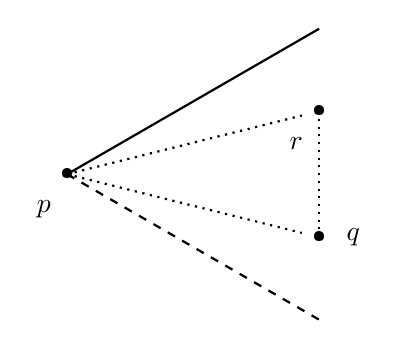
\begin{tikzpicture}[thick, scale=0.8]
        % \draw (0, -3) -- (0, 3) node[anchor=north west] {$y$};
        \draw (0, 0) -- (4, 2.309);
        \draw[dashed] (0, 0) -- (4, -2.309);
        \node[label=250:$p$] (p) at (0, 0) {\textbullet};
        \node[label=0:$q$] (q) at (4, -1) {\textbullet};
        \node[label=250:$r$] (r) at (4, 1) {\textbullet};
        \draw[dotted] (4, -1) -- (4, 1);
        \draw[dotted] (0, 0) -- (r);
        \draw[dotted] (0, 0) -- (q);
    \end{tikzpicture}
    \caption{A distância de $r$ até $q$ é menor do que a
    distância $p$ até $r$ e do que a distância $p$ até $q$.}
    \label{fig:parestatico:lcands}
\end{figure}